

\section{Trích xuất đặc trưng và tiền xử lý dữ liệu}

Dữ liệu thô từ các cảm biến ở dạng chuỗi thời gian chứa nhiều nhiễu nền và có số chiều lớn. Bước Trích xuất đặc trưng (Feature Extraction) giữ lại các đặc trưng tiêu biểu nhất về động lực học của máy giặt, tối ưu hóa không gian dữ liệu đầu vào cho mạng nơ-ron trên vi điều khiển.

\subsection{Thiết kế bộ lọc Mel tối ưu cho tín hiệu cơ khí}

Đối với dữ liệu âm thanh, đồ án chuyển đổi sang biểu diễn Năng lượng dải Mel (Mel-Frequency Energy - MFE). Mặc dù phổ Mel được dùng rộng rãi trong xử lý giọng nói, hệ thống tùy chỉnh cấu trúc này cho phân tích tiếng ồn cơ khí:

\begin{itemize}
    \item Tín hiệu âm thanh lấy mẫu ở tần số 8 kHz được phân khung kết hợp cửa sổ Hann để giảm hiện tượng rò rỉ phổ, sau đó áp dụng phép biến đổi Fourier nhanh 512 điểm với bước trượt 256 mẫu.

    \item Thay vì sử dụng 40 hoặc 128 dải Mel như các bài toán phân loại âm thanh tổng quát, hệ thống được tối ưu hóa xuống còn 13 dải lọc tam giác (13 Mel-bins). Các dải lọc tập trung mật độ cao ở vùng tần số thấp và trung — nơi phát ra tiếng ồn vận hành của động cơ và luồng nước — đồng thời giảm độ phân giải ở vùng tần số cao để loại bỏ nhiễu môi trường không mong muốn.

    \item Năng lượng tại mỗi dải Mel được tính theo thang logarit tự nhiên để mô phỏng đặc tính nén dải động của thính giác. Cách tiếp cận này làm nổi bật các dấu hiệu bất thường có biên độ nhỏ vốn dễ bị lấn át bởi nhiễu nền. Kết quả đầu ra là một vector 13 chiều cho mỗi khung âm thanh.
\end{itemize}

\begin{figure}[H]
    \centering
    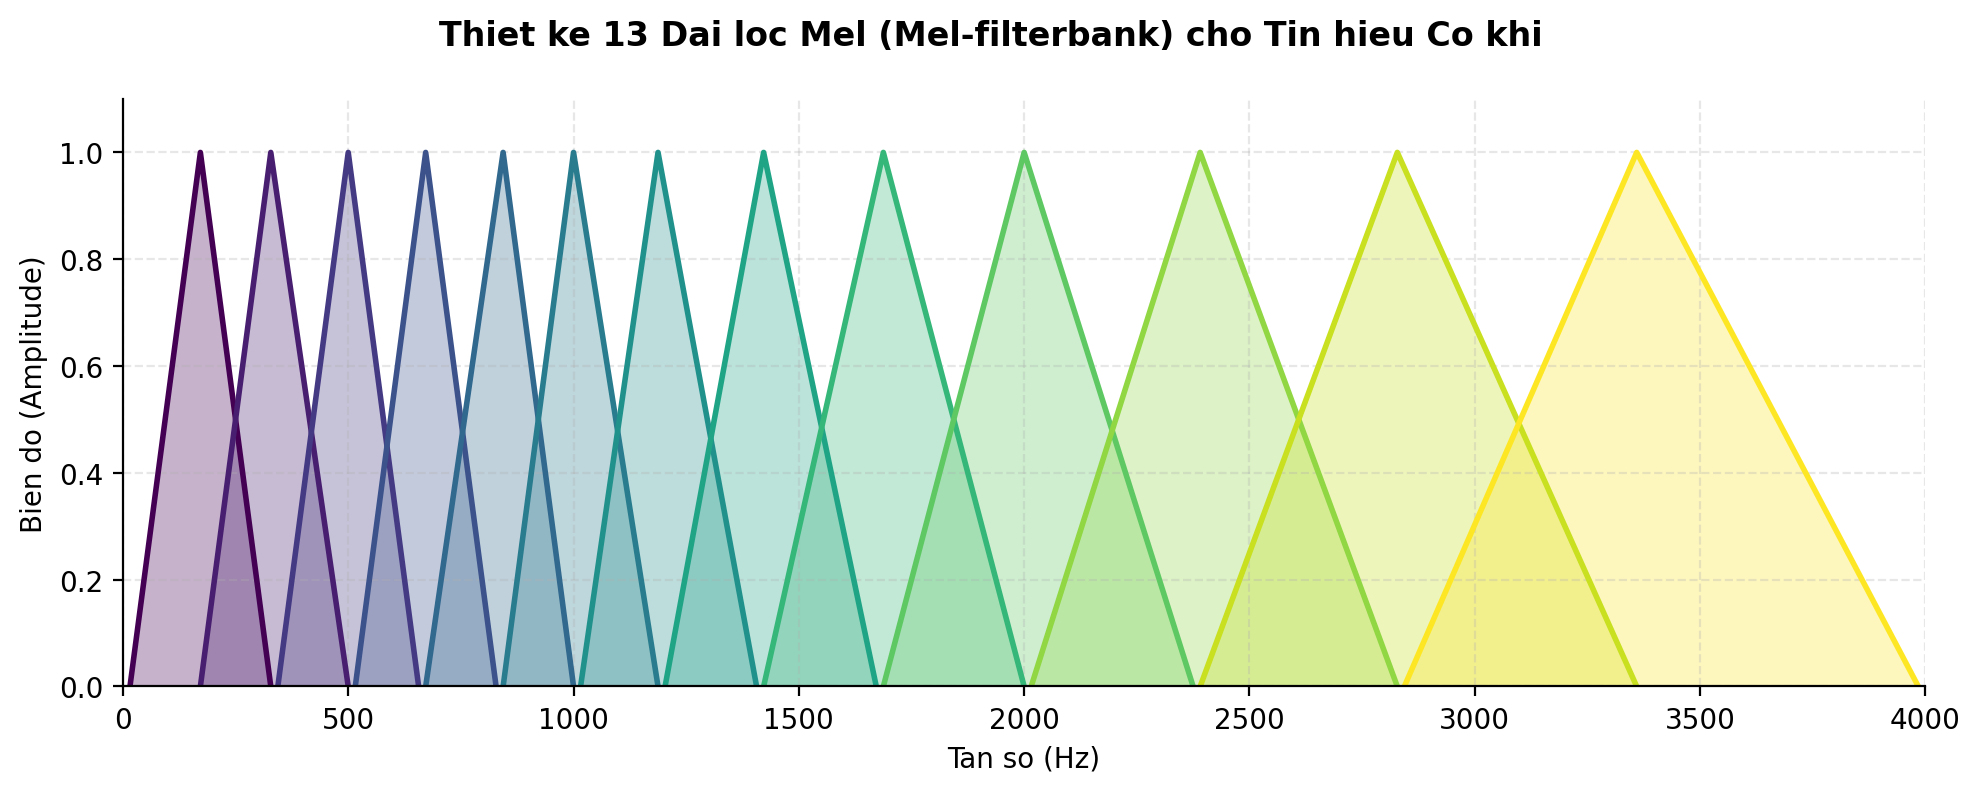
\includegraphics[width=0.9\linewidth]{chap3/image/fig_mel_filterbank.png}
    \caption[Cấu trúc 13 dải lọc Mel]{Trực quan hóa cấu trúc 13 dải lọc Mel tùy chỉnh được sử dụng trong hệ thống. Các bộ lọc hình tam giác được thiết kế phi tuyến, tập trung ở vùng tần số thấp (dưới 1000 Hz) để bóc tách tối đa âm thanh cơ học của máy giặt, đồng thời giảm phân giải ở dải tần cao để hạn chế nhiễu môi trường.}
    \label{fig:mel_filterbank}
\end{figure}

\subsection{Kỹ thuật đồng bộ hóa thuật toán xử lý giữa Python và Firmware C++}

Khi phát triển TinyML, sai lệch biểu diễn (Representation Mismatch) là vấn đề thường gặp. Trong giai đoạn thử nghiệm đầu, mô hình mạng nơ-ron tự mã hóa đạt độ chính xác cao trên Python nhưng sinh ra cảnh báo giả khi triển khai lên vi điều khiển Seeed Studio XIAO ESP32-S3.

Nguyên nhân là sự khác biệt trong tính toán dấu phẩy động: Python sử dụng thư viện \texttt{librosa} với độ chính xác kép (Float64), trong khi firmware C++ thực thi các hàm FFT bằng tập lệnh vector trên kiến trúc Xtensa LX7 chỉ hỗ trợ Float32, kết hợp với mảng lọc tĩnh \texttt{MEL\_FB} tự định nghĩa. Sai số tích lũy qua 13 dải tần đã làm thay đổi phân phối của vector đặc trưng đầu vào so với lúc huấn luyện.

Để khắc phục, đồ án thiết kế lại luồng trích xuất đặc trưng theo cơ chế nhất quán:

\begin{enumerate}
    \item Loại bỏ sự phụ thuộc vào \texttt{librosa}. Mã nguồn Python được viết lại để tính toán FFT và Mel-filterbank bằng các phép toán ma trận NumPy cơ bản, mô phỏng chính xác logic làm tròn số và mảng \texttt{MEL\_FB} của mã nguồn C++.

    \item Áp dụng hệ số nhân tĩnh (Static Scaling Factor) và giới hạn dải năng lượng trong khoảng $[-80, 0]$ dB một cách đồng nhất trên cả hai môi trường.
\end{enumerate}

Phương pháp định hướng firmware (Firmware-Driven Data Pipeline) này đảm bảo nguyên tắc "Train as you deploy", giúp phân phối dữ liệu tại máy chủ huấn luyện và thiết bị biên trùng khớp nhau.

\subsection{Xử lý dữ liệu ngoại lai cho tín hiệu rung động}

Đối với cảm biến gia tốc ADXL345, 6 đặc trưng thống kê được trích xuất bao gồm giá trị hiệu dụng (RMS) và phương sai của ba trục X, Y, Z. Dữ liệu chấn động của máy giặt chứa nhiều ngoại lai (Outliers) mang tính nhất thời, chẳng hạn như tiếng cúc áo va đập vào lồng giặt hoặc sự xô lệch đột ngột của tải trọng.

Nếu áp dụng MinMax Scaling tiêu chuẩn, một gai nhiễu đơn lẻ có thể làm thay đổi toàn bộ dải cực trị, nén 99\% dữ liệu bình thường vào một dải biên độ hẹp và mất khả năng phân biệt các biến động nhỏ. Do đó, đồ án sử dụng kỹ thuật xử lý hỗn hợp (Hybrid Scaling):

\begin{enumerate}
    \item \textbf{Cắt xén ngoại lai (Clipping):} Đối với phương sai trục X và trục Y (nhạy cảm với va đập), thuật toán xác định ngưỡng cắt tại phân vị thứ 99 của tập huấn luyện và giới hạn các giá trị vượt ngưỡng về mức biên này (99th Percentile Clipping). Riêng phương sai trục Z được giữ nguyên dải giá trị ban đầu, vì đây là đặc trưng quyết định để phân loại trạng thái ba trạng thái.

    \item \textbf{Chuẩn hóa (Scaling):} Dữ liệu sau khi qua bộ lọc Clipping được chuẩn hóa bằng RobustScaler. Đồ án mở rộng khoảng phân vị tính toán lên $(10, 90)$ thay vì IQR tiêu chuẩn $(25, 75)$ để bao quát tốt hơn dải động của cảm biến \cite{ref_3_robust_scaler}. Đồng thời, một hệ số bù tối thiểu $0.002$ được cộng thêm vào mẫu số để tránh lỗi chia cho 0 khi máy giặt ở pha tĩnh (GENTLE), đảm bảo tính ổn định số học của hệ thống.
\end{enumerate}

% ==============================================================================
% DANH MỤC TÀI LIỆU THAM KHẢO TRÍCH DẪN (MỤC 3.2)
% ==============================================================================
% \bibitem{ref_3_robust_scaler} P. J. Rousseeuw and A. M. Leroy, "Robust Regression and Outlier Detection," John Wiley & Sons, 2005.


% ==============================================================================
% HẾT MỤC 3.2
% ==============================================================================


% --- Hết chương 3 mục 2 ---
